%%==================================================
%% chapter04.tex for SJTU Master Thesis
%% Encoding: UTF-8
%%==================================================

\chapter{算法在CUDA平台的实现}
  本实习在Ubuntu 14.04.1 LTS上实现了Hessian-Affine的CUDA版本,并且通过不同分辨率的图片测试出了算法中各个函数的加速比,以及整体的加速比。
  \subparagraph{测试数据}
    由于本算法会被两个变量影响性能:
    \begin{enumerate}
      \item 图像大小
      \item 图像复杂度
    \end{enumerate}
    \par
    因此,为了测试加速比,我选用了500张分辨率为1024*768的图像作测试,由于以特征点数量作为因变量,时间作为参变量,以上图片均来自Oxford 5k数据集。
  \subparagraph{数据流}
    本算法的数据流简要如下:生成尺度空间->在尺度空间中计算每个点的Hessian相应->精确定位特征点->寻找仿射标准形->计算SIFT描述子。在这个算法中,每个部分的都可以并行,但是并行的粒度不同,导致了CUDA的加速比不同。
    \par
    以下是算法中主要函数函数的加速比:
    \begin{figure}[htp]
      \centering
      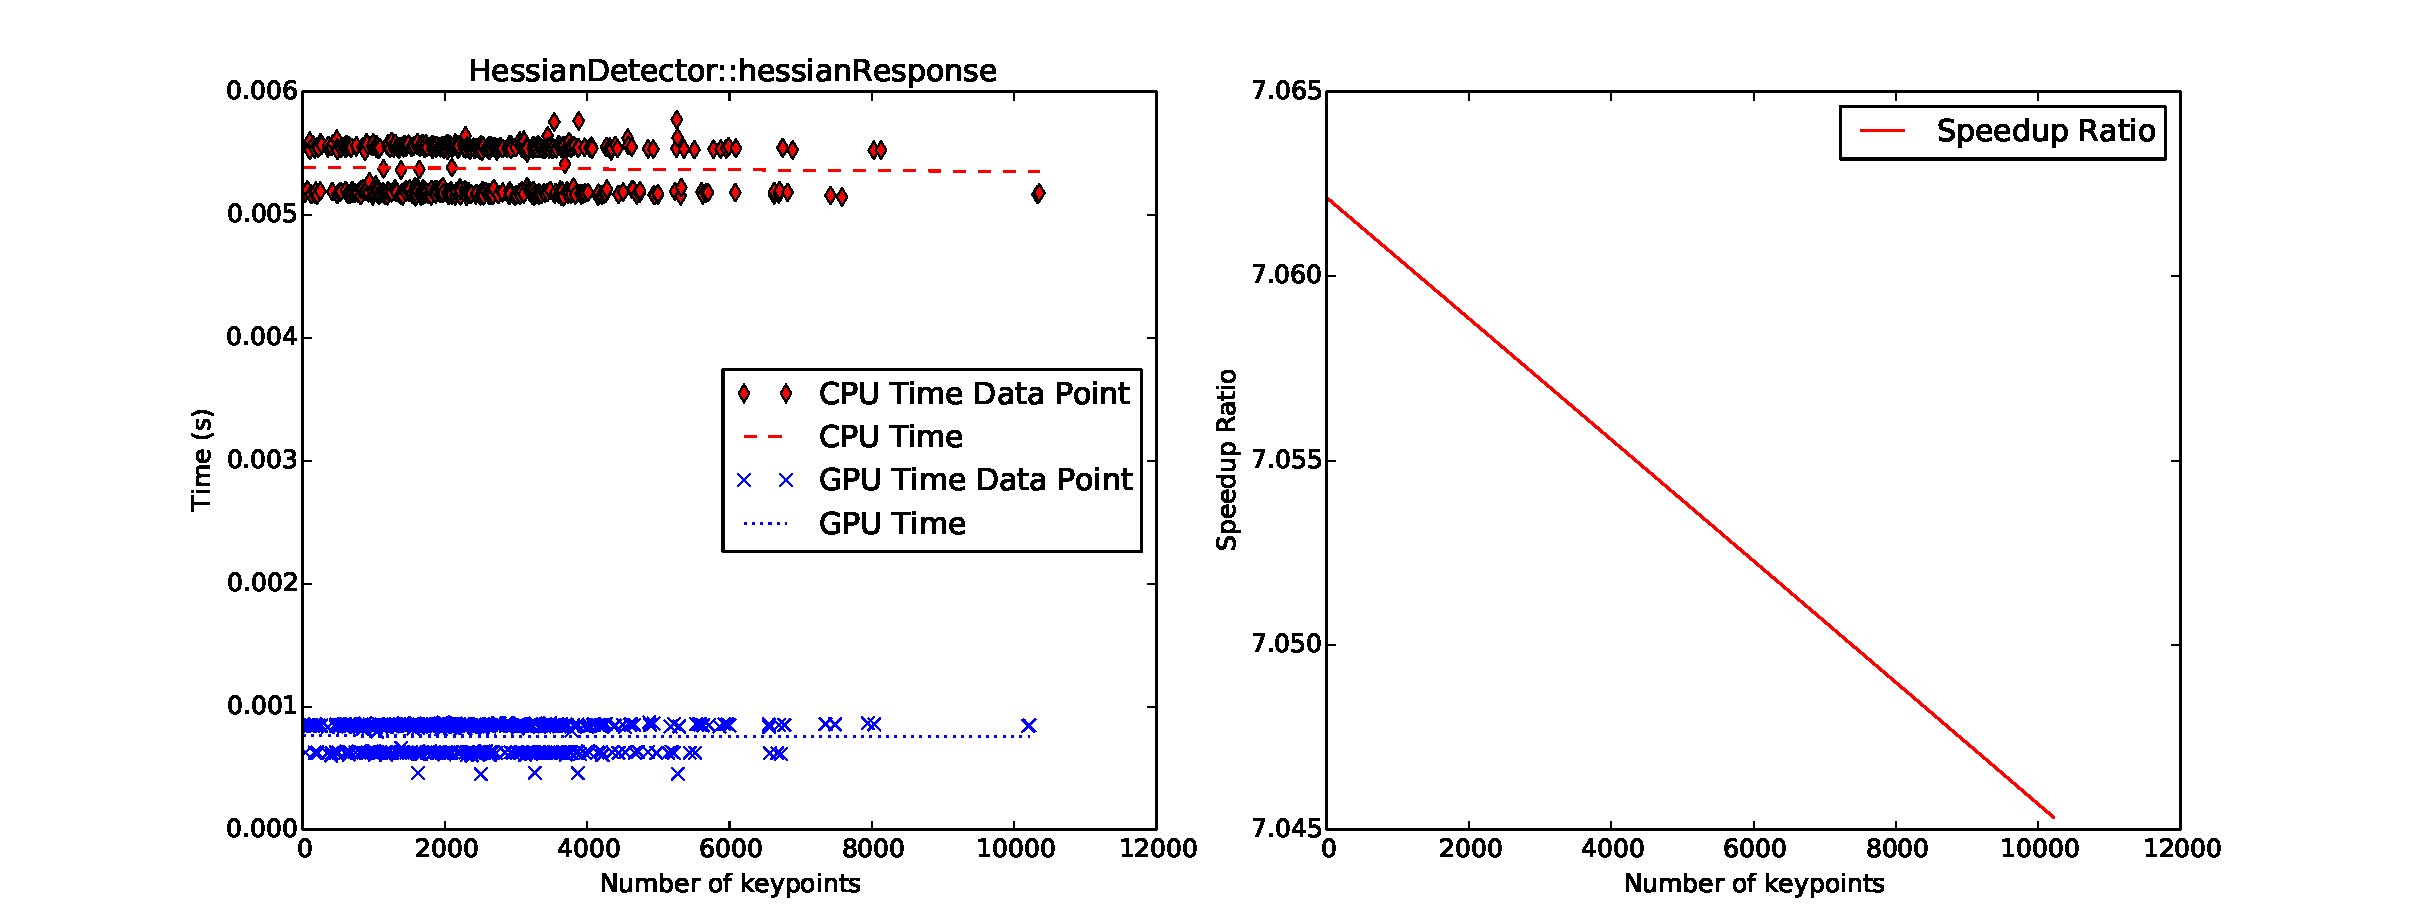
\includegraphics[width=1\textwidth]{chap4/hessianResponse}
      \caption{hessianResponse函数的加速比}
    \end{figure}
    \begin{figure}[htp]
      \centering
      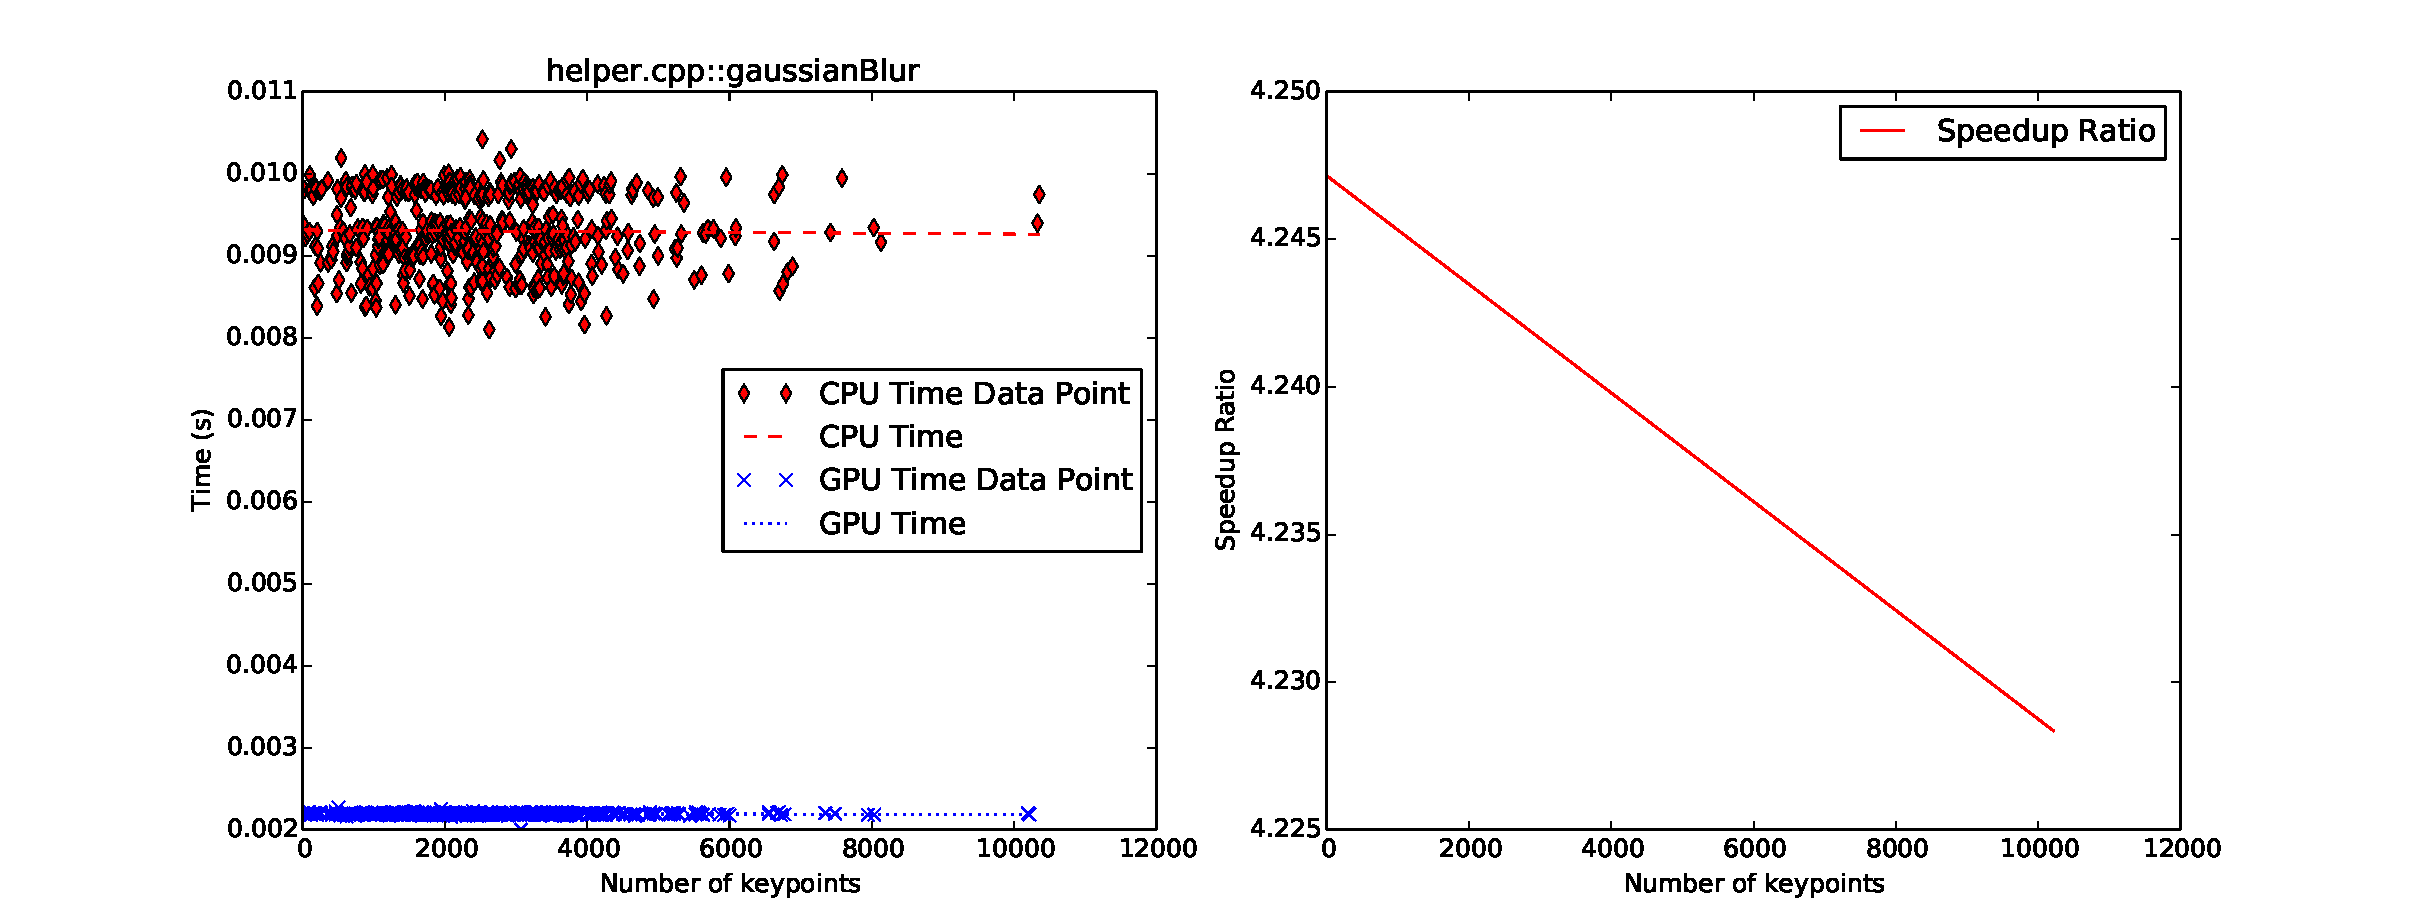
\includegraphics[width=1\textwidth]{chap4/gaussianBlur}
      \caption{gaussianBlur函数的加速比}
    \end{figure}
    \begin{figure}[htp]
      \centering
      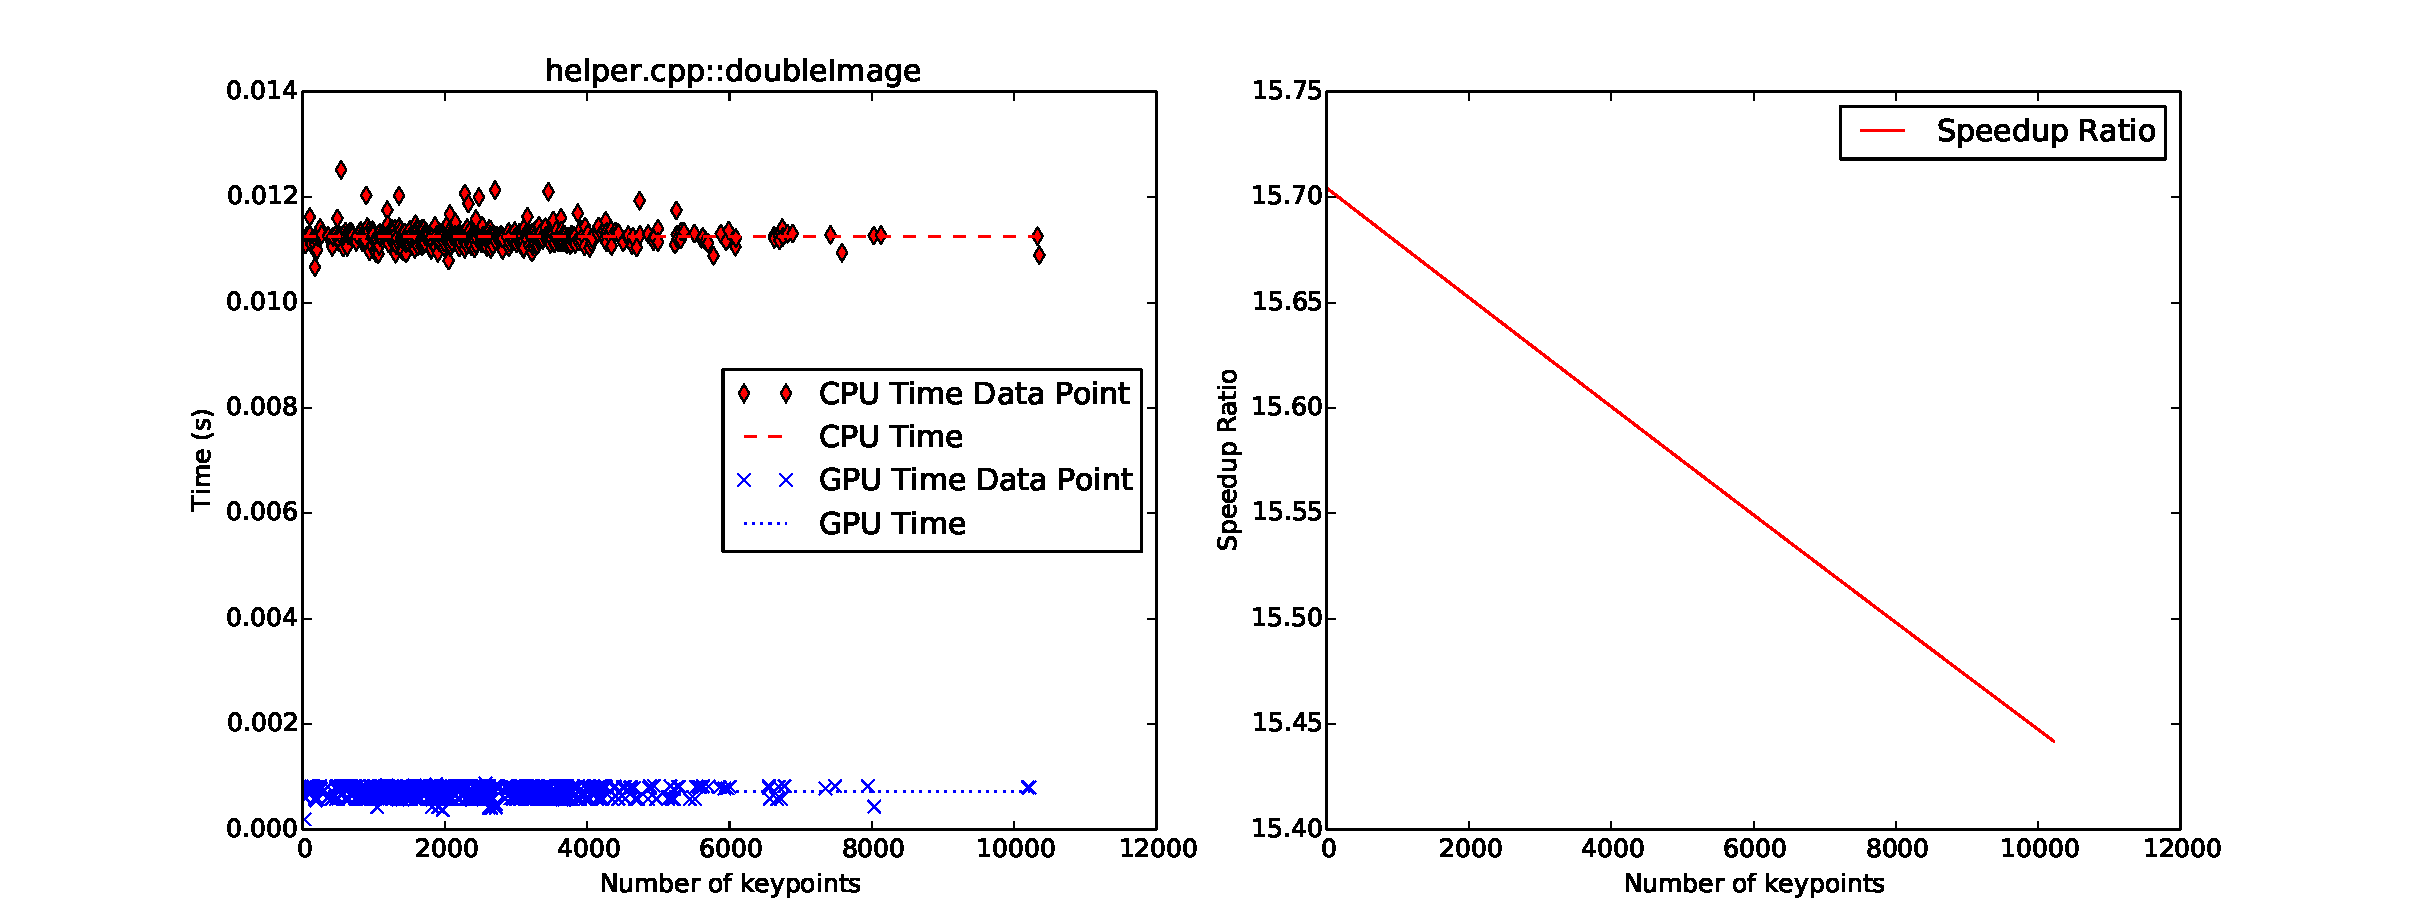
\includegraphics[width=1\textwidth]{chap4/doubleImage}
      \caption{doubleImage函数的加速比}
    \end{figure}
    \begin{figure}[htp]
      \centering
      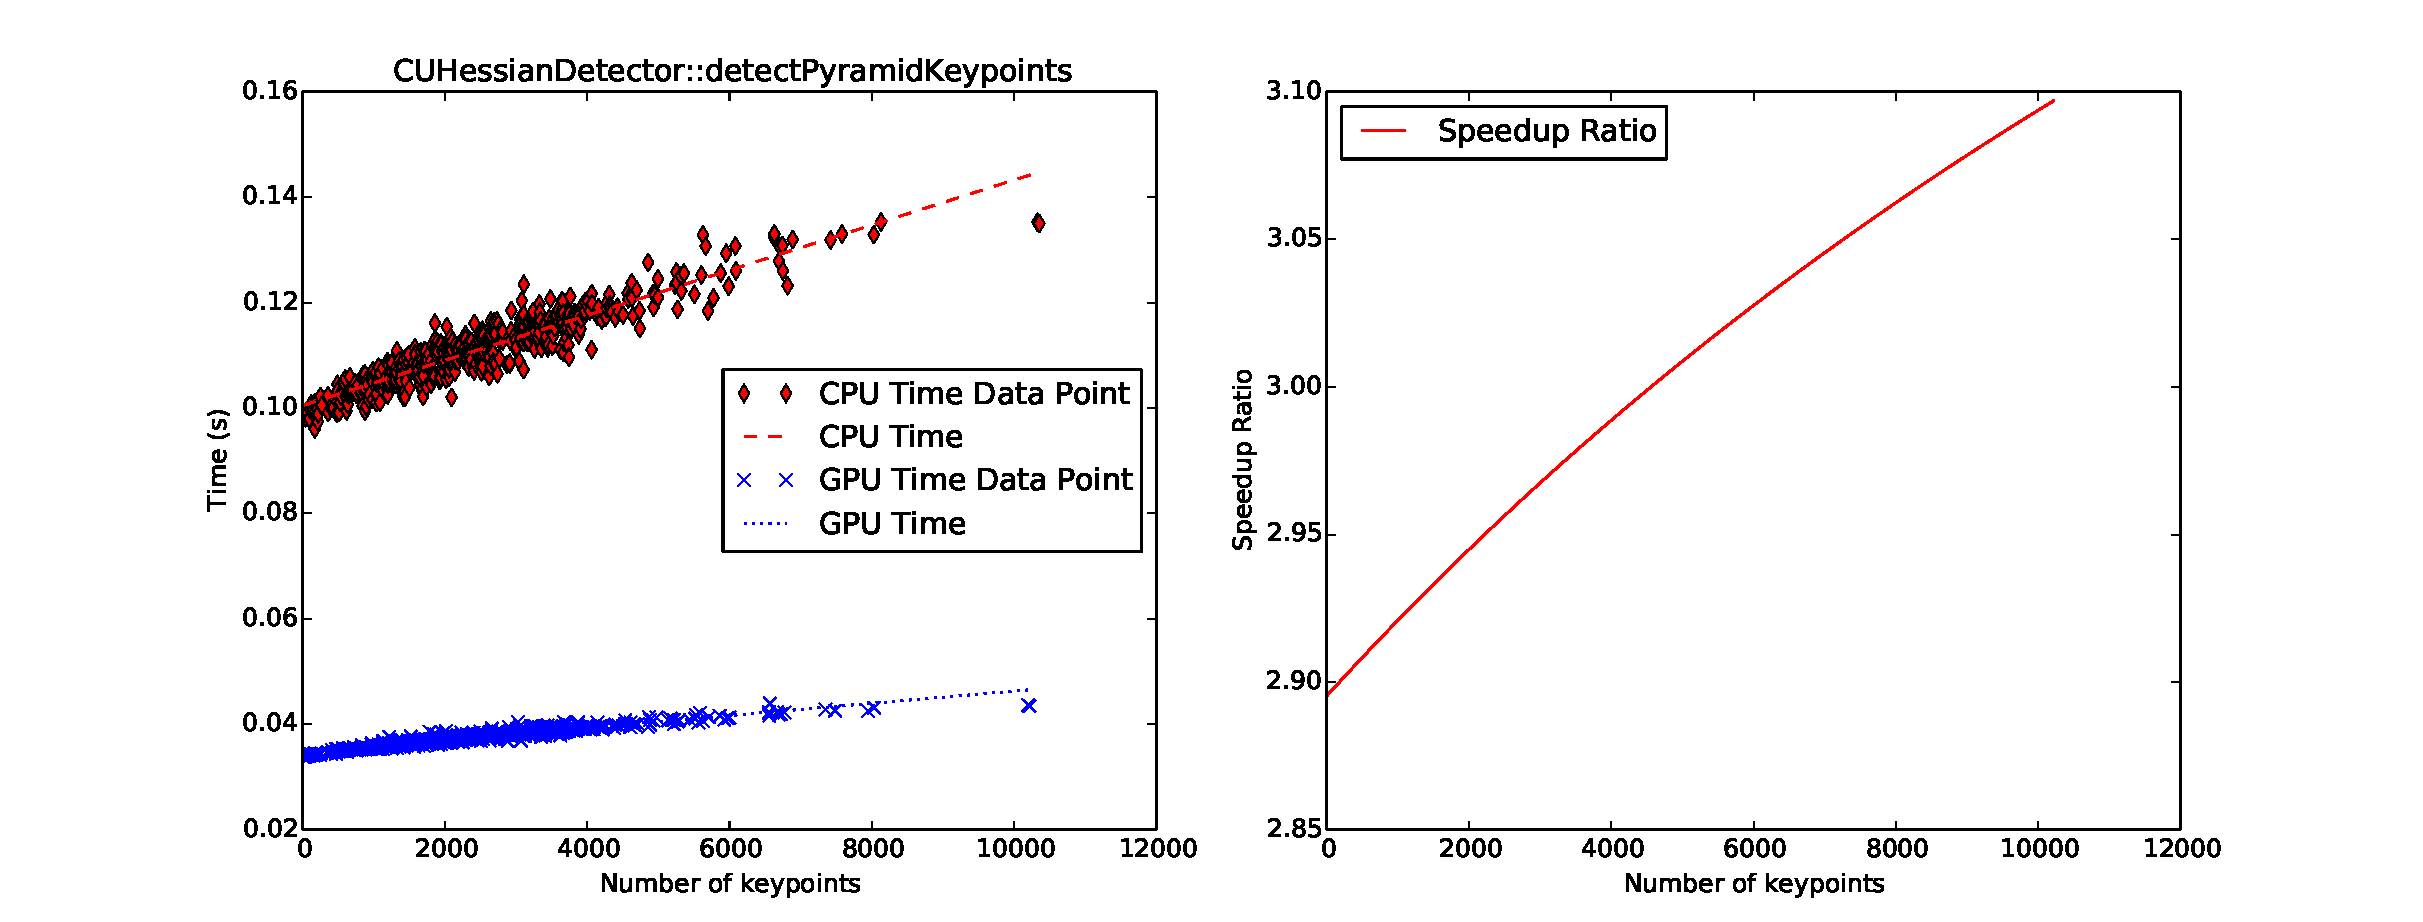
\includegraphics[width=1\textwidth]{chap4/detectPyramid}
      \caption{detectPyramid函数的加速比}
    \end{figure}
    以及总体的加速比:
    \begin{figure}[htp]
      \centering
      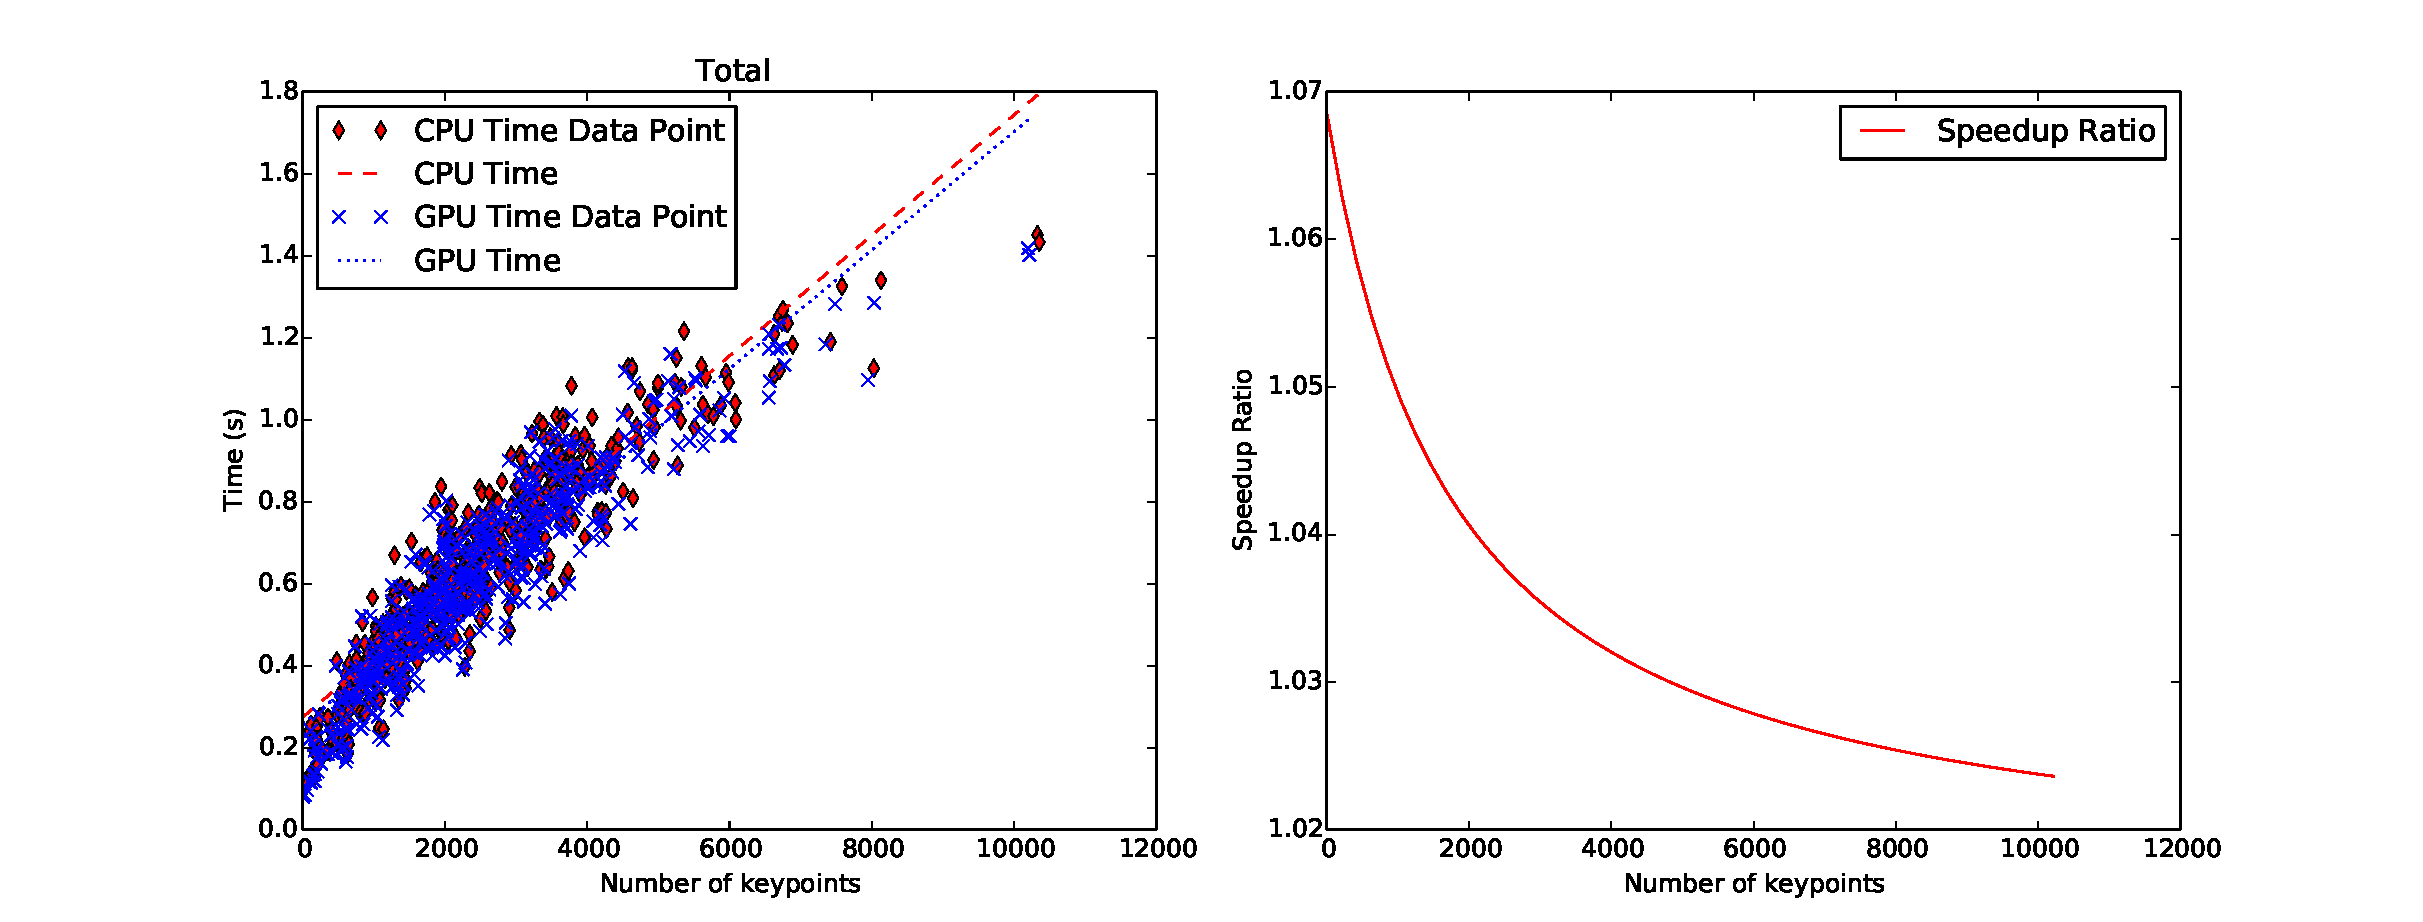
\includegraphics[width=1\textwidth]{chap4/Total}
      \caption{总体的加速比}
    \end{figure}
  \subsection*{结论}
    在这次实习中,实现了Hessian-Affine算法的GPU版本,但是由于数据与算法特性的影响,在运算中存在大量的迭代,并且由于GPU不支持计算能力3.5添加的新特性:动态并行化。虽然在细粒度并行运算速度很快,在某些运算上的加速比达到了10倍以上;但是GPU缺乏粗粒度的并行能力,导致CPU不得不频繁通过PCI-E总线控制GPU的运作,加之本次的实验平台PCI-E版本为1.0,总带宽为16Gbps,实际带宽大约为1GB/s,极大的降低了算法的性能。
    \par
    本算法还有继续改进的空间,在本次实验平台下,可以通过重构算法结构来获得更大的性能提升。
